\documentclass[aspectratio=169,10pt]{beamer}

% --- Typography & Encoding ---
\usepackage[T1]{fontenc}
\usepackage{lmodern}
\usepackage{booktabs}
\usepackage{tikz}
\usepackage{amsmath}
\usepackage{totcount}
\usetikzlibrary{arrows.meta, positioning, calc, shapes.misc, patterns, backgrounds, shapes.geometric}

% --- Theme Setup ---
\usetheme{default}
\useinnertheme{rectangles}
\setbeamertemplate{navigation symbols}{}
\setbeamertemplate{blocks}[rounded][shadow=false]

% --- Hadron Energy Brand Palette ---
\definecolor{HadronDark}{RGB}{33, 43, 54}       % Deep Slate/Navy
\definecolor{HadronBlue}{RGB}{0, 122, 204}      % Corporate Blue
\definecolor{HadronLight}{RGB}{245, 247, 250}   % Off-white background

% Status Colors
\definecolor{StatusRed}{RGB}{220, 53, 69}
\definecolor{StatusYellow}{RGB}{255, 193, 7}
\definecolor{StatusGreen}{RGB}{40, 167, 69}
\definecolor{StatusDark}{RGB}{52, 58, 64}
\definecolor{StatusOrange}{RGB}{253, 126, 20}

% --- Beamer Color Customization ---
\setbeamercolor{background canvas}{bg=white}
\setbeamercolor{frametitle}{bg=white, fg=HadronDark}
\setbeamercolor{title}{fg=white}
\setbeamercolor{subtitle}{fg=HadronBlue}
\setbeamercolor{structure}{fg=HadronBlue}
\setbeamercolor{itemize item}{fg=HadronBlue}
\setbeamercolor{itemize subitem}{fg=HadronDark}

% Block styling
\setbeamercolor{block title}{bg=HadronDark, fg=white}
\setbeamercolor{block body}{bg=HadronLight, fg=black}

% Font Sizes
\setbeamerfont{frametitle}{size=\large,series=\bfseries}
\setbeamerfont{block title}{size=\normalsize,series=\bfseries}

% --- Custom Graphics Definitions ---
\newcommand{\insertheaderlogo}{%
    % Ensure this image exists in your media folder, or comment it out
    \includegraphics[width=2.5cm, keepaspectratio]{media/hadron_logo.png}%
}

\newcommand{\statusbadge}[2]{%
    \tikz[baseline=(node.base)]{
        \node[fill=#1, text=white, rounded corners=3pt, inner sep=5pt, font=\bfseries\footnotesize, align=center, minimum width=2.5cm] (node) {#2};
    }%
}

% --- HEADER TEMPLATE ---
\setbeamertemplate{frametitle}{
    \nointerlineskip
    \begin{beamercolorbox}[wd=\paperwidth,ht=1.3cm,dp=0.6ex,leftskip=0.5cm,rightskip=0.5cm,sep=0cm,vmode]{frametitle}
        \centering
        \begin{minipage}[c][1.3cm][c]{\dimexpr\paperwidth-1cm\relax}
            \begin{minipage}[c]{0.72\textwidth}
                \raggedright
                \usebeamerfont{frametitle}\insertframetitle
            \end{minipage}%
            \hfill
            \begin{minipage}[c]{0.23\textwidth}
                \raggedleft
                \insertheaderlogo
            \end{minipage}
        \end{minipage}
    \end{beamercolorbox}
    \nointerlineskip
    {\color{HadronBlue}\hrule height 1pt}
}

% --- FOOTER TEMPLATE ---
\setbeamertemplate{footline}{
    \leavevmode%
    \hbox{%
    \begin{beamercolorbox}[wd=.333333\paperwidth,ht=2.25ex,dp=1ex,left]{author in head/foot}%
        \hspace*{2ex} \textcolor{gray}{\insertshortauthor}
    \end{beamercolorbox}%
    \begin{beamercolorbox}[wd=.333333\paperwidth,ht=2.25ex,dp=1ex,center]{title in head/foot}%
        \textcolor{gray}{\textbf{RG 1.203 \& BEPU METHODOLOGY}}
    \end{beamercolorbox}%
    \begin{beamercolorbox}[wd=.333333\paperwidth,ht=2.25ex,dp=1ex,right]{date in head/foot}%
        \textcolor{gray}{\insertframenumber{} / \inserttotalframenumber}\hspace*{2ex} 
    \end{beamercolorbox}}%
}

% --- Metadata ---
\title{Regulatory Guide 1.203 \& BEPU}
\subtitle{Transient and Accident Analysis Methods}
\author{Lander Ibarra}
\institute{Hadron Energy}
\date{\today}

\begin{document}

% ==========================================
% SLIDE 1: TITLE PAGE
% ==========================================
\begin{frame}[plain]
    \begin{tikzpicture}[remember picture,overlay]
        \fill[HadronDark] (current page.north west) rectangle (current page.south east);
        \node[anchor=north east] at (current page.north east) {
            \begin{tikzpicture}
                \fill[white] (0,0) rectangle (-4.0cm, -1.6cm); 
                \node[anchor=center] at (-2.0cm, -0.8cm) {
                    \includegraphics[width=3.0cm, keepaspectratio]{media/hadron_logo.png}
                };
            \end{tikzpicture}
        };
        \draw[HadronBlue, thick] ([yshift=-1.6cm]current page.north west) -- ([yshift=-1.6cm]current page.north east);
    \end{tikzpicture}
    
    \vspace{2.0cm} 
    \begin{center}
        \textcolor{HadronBlue}{\small \textbf{ENGINEERING \& LICENSING BRIEFING}} \\[0.5em]
        {\Huge \textbf{\textcolor{white}{Regulatory Guide 1.203}}}\\
        {\Large \textbf{\textcolor{white}{Best Estimate Plus Uncertainty (BEPU)}}}
        
        \vspace{0.5cm}
        \textcolor{gray}{Evaluation Model Development and Assessment Process}
        
        \vspace{1.5cm}
        \begin{columns}
            \column{0.5\textwidth}
            \raggedright
            \textcolor{gray}{\small PREPARED BY:}\\
            \textcolor{white}{\textbf{Lander Ibarra}}
            
            \column{0.5\textwidth}
            \raggedleft
            \textcolor{gray}{\small DATE:}\\
            \textcolor{white}{\textbf{\insertdate}}
        \end{columns}
    \end{center}
\end{frame}

\setcounter{framenumber}{0}

% ==========================================
% SLIDE 2: EXECUTIVE SUMMARY
% ==========================================
\begin{frame}[t]{Executive Summary}
    \vspace{0.5em}
    \begin{columns}[T,onlytextwidth]
        \column{0.65\textwidth}
        \begin{block}{Briefing Objectives}
            \begin{itemize}
                \item \textbf{Regulatory Framework:} Overview of the EMDAP framework outlined in NRC RG 1.203.
                \item \textbf{Statistical Rigor:} Define the best-practice approach for establishing Probability Density Functions (PDFs).
                \item \textbf{Combination of Uncertainties:} How individual parameter variations are mathematically aggregated to prove safety limits.
            \end{itemize}
        \end{block}

        \begin{block}{Key Deliverables}
            \begin{itemize}
                \item Traceable, documented basis for statistical inputs.
                \item Computation of valid 95/95 safety bounds.
            \end{itemize}
        \end{block}

        \column{0.32\textwidth}
        \centering
        \textbf{Methodology Focus}
        \vspace{1em}
        \statusbadge{StatusGreen}{1. PIRT Process}
        \vspace{0.5em}
        \statusbadge{StatusYellow}{2. Data Sourcing}
        \vspace{0.5em}
        \statusbadge{StatusRed}{3. Combination}
    \end{columns}
\end{frame}

% ==========================================
% SLIDE 3: REGULATORY SHIFT
% ==========================================
\begin{frame}[t]{Regulatory Shift: BEPU \& RG 1.203}
    \begin{columns}[T,onlytextwidth]
        \column{0.55\textwidth}
        \textbf{The BEPU Philosophy:}
        Historically, safety codes used punitive, worst-case deterministic assumptions (e.g., Appendix K). The NRC now encourages \textbf{Best Estimate Plus Uncertainty (BEPU)} approaches, using realistic physics paired with rigorous statistical quantification.

        \vspace{1em}
        \textbf{The Evaluation Model (EM):}
        Under RG 1.203, an Evaluation Model is not just a computer code. It is the entire suite of:
        \begin{itemize} \small
            \item The physical code (e.g., RELAP, TRACE, VERA).
            \item The spatial nodalization scheme.
            \item The numerical solution techniques.
            \item \textbf{The specific uncertainty methodology.}
        \end{itemize}

        \column{0.42\textwidth}
        \begin{block}{Why use BEPU?}
            \begin{itemize} \small
                \item Recovers trapped safety margin.
                \item Allows for reactor power uprates.
                \item Improves operational flexibility without compromising the licensing basis.
            \end{itemize}
        \end{block}
    \end{columns}
\end{frame}

% ==========================================
% SLIDE 4: THE EMDAP FLOW (TIKZ)
% ==========================================
\begin{frame}[t]{The 4 Elements of EMDAP}
    \textbf{Evaluation Model Development and Assessment Process}
    \vspace{0.5cm}
    \begin{center}
    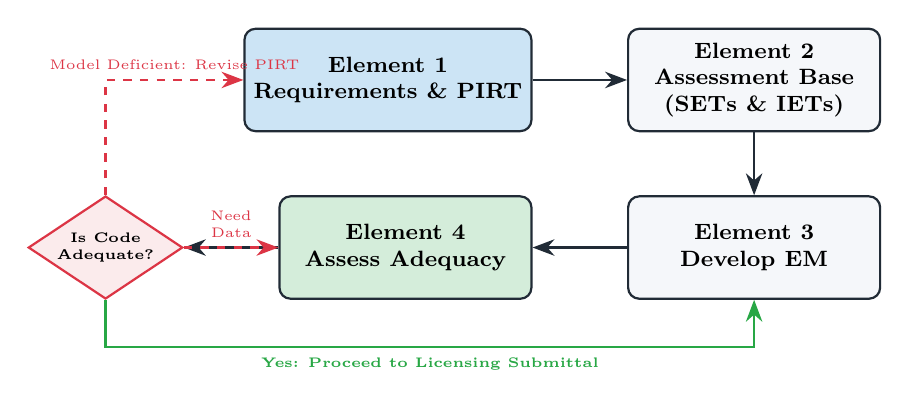
\begin{tikzpicture}[
        node distance=0.8cm and 1.2cm,
        box/.style={rectangle, draw=HadronDark, fill=HadronLight, thick, rounded corners, minimum width=3.2cm, minimum height=1.3cm, align=center, font=\footnotesize\bfseries},
        decision/.style={diamond, draw=StatusRed, fill=StatusRed!10, thick, aspect=1.5, align=center, font=\tiny\bfseries, inner sep=1pt},
        arrow/.style={-{Stealth[scale=1.2]}, thick, HadronDark},
        feedback/.style={-{Stealth[scale=1.2]}, dashed, thick, StatusRed}
    ]
        
        % Nodes
        \node[box, fill=HadronBlue!20] (e1) {Element 1\\Requirements \& PIRT};
        \node[box, right=of e1] (e2) {Element 2\\Assessment Base\\(SETs \& IETs)};
        \node[box, below=of e2] (e3) {Element 3\\Develop EM};
        \node[box, left=of e3, fill=StatusGreen!20] (e4) {Element 4\\Assess Adequacy};
        
        \node[decision, left=of e4] (adeq) {Is Code\\Adequate?};
        
        % Arrows
        \draw[arrow] (e1) -- (e2);
        \draw[arrow] (e2) -- (e3);
        \draw[arrow] (e3) -- (e4);
        \draw[arrow] (e4) -- (adeq);
        
        % Output
        \draw[arrow, StatusGreen] (adeq.south) |- ++(0,-0.6) -| node[pos=0.25, below, font=\tiny\bfseries] {Yes: Proceed to Licensing Submittal} (e3.south);
        
        % Feedback Loops
        \draw[feedback] (adeq.north) |- node[pos=0.75, above, font=\tiny] {Model Deficient: Revise PIRT} (e1.west);
        \draw[feedback] (adeq.east) -- node[above, font=\tiny, align=center] {Need\\Data} (e4.west);
        
    \end{tikzpicture}
    \end{center}
    
    \vspace{0.5em}
    \begin{itemize} \small
        \item \textbf{Iterative Strictness:} RG 1.203 requires that if the code cannot predict reality within established uncertainty bounds, developers must loop back to fix the code, gather more experimental data, or revise the PIRT.
    \end{itemize}
\end{frame}

% ==========================================
% SLIDE 5: STEP 1: PIRT OVERVIEW
% ==========================================
\begin{frame}[t]{Step 1: Establish Requirements (PIRT)}
    \textbf{Phenomena Identification and Ranking Table (PIRT):}
    Before assigning math to uncertainties, a panel of experts determines what parameters actually affect the Figures of Merit (e.g., Peak Cladding Temperature).

    \vspace{1em}
    \begin{columns}[T,onlytextwidth]
        \column{0.30\textwidth}
        \begin{block}{1. Identify}
            List every conceivable parameter and physical phenomenon that could affect the transient.
        \end{block}

        \column{0.30\textwidth}
        \begin{block}{2. Rank}
            Rank by Importance (High, Medium, Low) and Knowledge Level (Known, Partially Known, Unknown).
        \end{block}
        
        \column{0.30\textwidth}
        \begin{block}{3. Focus}
            Only build rigorous PDFs for \textbf{High Importance} parameters to optimize computational resources.
        \end{block}
    \end{columns}
    
    \vspace{1.5em}
    \centering
    \statusbadge{HadronDark}{Low Importance = Held at Nominal or Deterministic Biased}
\end{frame}

% ==========================================
% SLIDE 6: PIRT EXECUTION TABLE
% ==========================================
\begin{frame}[t]{Element 1: PIRT Execution Example}
    \vspace{1em}
    \centering
    \begin{table}[]
        \small
        \begin{tabular}{@{}llcl@{}}
            \toprule
            \textbf{Component} & \textbf{Phenomenon} & \textbf{Importance} & \textbf{Knowledge Level} \\ \midrule
            Core & Post-accident Heat Transfer & \textcolor{StatusRed}{\textbf{High}} & \textcolor{StatusYellow}{\textbf{Medium}} \\
            Core & Decay Heat Profile & \textcolor{StatusRed}{\textbf{High}} & High \\
            Downcomer & 3D Flow Mixing & \textcolor{StatusRed}{\textbf{High}} & \textcolor{StatusRed}{\textbf{Low}} \\
            Pressurizer & Flashing & Low & High \\ \bottomrule
        \end{tabular}
    \end{table}

    \vspace{0.5em}
    \begin{columns}[T]
        \column{0.8\textwidth}
        \begin{block}{Actionable Output}
            High Importance + Low/Medium Knowledge = \textbf{Knowledge Gap}. EMDAP requires focusing resources, experimental testing, and EM development specifically on these gaps.
        \end{block}
    \end{columns}
\end{frame}

% ==========================================
% SLIDE 7: ELEMENTS 2 & 3
% ==========================================
\begin{frame}[t]{Elements 2 \& 3: Data and Code Development}
    \begin{columns}[T,onlytextwidth]
        \column{0.48\textwidth}
        \textbf{Element 2: Assessment Base}
        \begin{itemize}
            \item Gather experimental data to validate the phenomena identified in the PIRT.
            \item \textbf{Separate Effects Tests (SET):} Isolate a single phenomenon (e.g., heat transfer in a single heated pipe).
            \item \textbf{Integral Effects Tests (IET):} Scaled-down facilities that simulate the whole plant (e.g., LOFT, ROSA) to capture system interactions.
        \end{itemize}

        \column{0.48\textwidth}
        \textbf{Element 3: Develop the EM}
        \begin{itemize}
            \item Build the mathematical models, spatial nodalization schemes, and numerical solvers.
            \item Establish the code architecture and closure relations.
            \item \textbf{Scaling:} Ensure the code scales properly from a small test facility to a full-size commercial reactor.
        \end{itemize}
    \end{columns}
\end{frame}

% ==========================================
% SLIDE 8: ELEMENT 4
% ==========================================
\begin{frame}[t]{Element 4: Assess EM Adequacy}
    How do we prove the code works? RG 1.203 requires a dual-pronged approach:

    \vspace{0.5em}
    \centering
    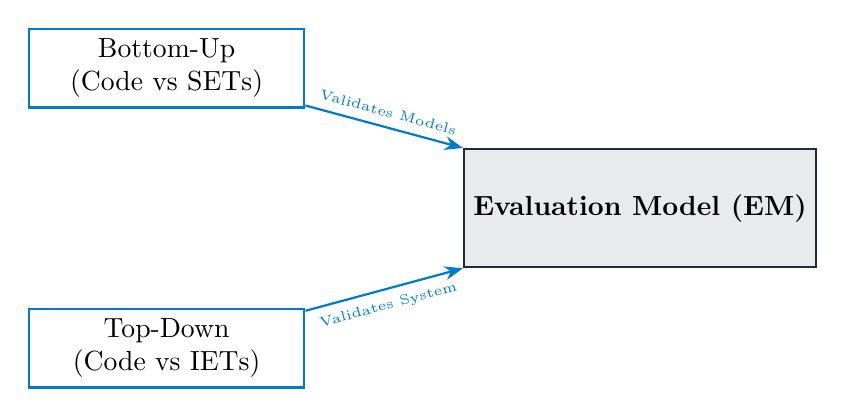
\begin{tikzpicture}[
        node distance=0.5cm and 2cm,
        box/.style={rectangle, draw=HadronBlue, fill=white, thick, minimum width=3.5cm, minimum height=1cm, align=center},
        mainbox/.style={rectangle, draw=HadronDark, fill=HadronDark!10, thick, minimum width=4cm, minimum height=1.5cm, align=center, font=\bfseries}
    ]
        
        \node[mainbox] (code) {Evaluation Model (EM)};
        
        \node[box, above left=of code] (bu) {Bottom-Up\\(Code vs SETs)};
        \node[box, below left=of code] (td) {Top-Down\\(Code vs IETs)};
        
        \draw[-{Stealth}, thick, HadronBlue] (bu) -- node[above, font=\tiny, sloped] {Validates Models} (code.north west);
        \draw[-{Stealth}, thick, HadronBlue] (td) -- node[below, font=\tiny, sloped] {Validates System} (code.south west);
        
    \end{tikzpicture}
    
    \vspace{1em}
    \begin{itemize}
        \item \textbf{Bottom-Up:} Prove individual closure equations work using Separate Effects Tests.
        \item \textbf{Top-Down:} Prove the code handles complex system interactions using Integral Effects Tests and actual plant transient data.
    \end{itemize}
\end{frame}

% ==========================================
% SLIDE 9: DEFINING PDFs
% ==========================================
\begin{frame}[t]{Defining Probability Density Functions (PDFs)}
    \begin{columns}[T,onlytextwidth]
        \column{0.55\textwidth}
        \textbf{The Core of BEPU Licensing:}
        Defining the PDFs is arguably the most highly scrutinized step in a BEPU submittal. 
        
        \vspace{1em}
        \textbf{The Risk of Flawed Inputs:}
        If your input distributions are flawed, your 95/95 safety limits are invalid. The NRC expects a rigorous, traceable, and heavily documented basis for every single distribution fed into a statistical engine.

        \column{0.40\textwidth}
        \begin{block}{Three Data Categories}
            \begin{enumerate}
                \item Manufacturing Tolerances
                \item Operating Conditions
                \item Modeling Uncertainties
            \end{enumerate}
        \end{block}
    \end{columns}
\end{frame}

% ==========================================
% SLIDE 10: PDF SCHEMATIC (TIKZ)
% ==========================================
\begin{frame}[t]{Defining Input Distributions (PDFs)}
    \vspace{0.5em}
    \begin{center}
    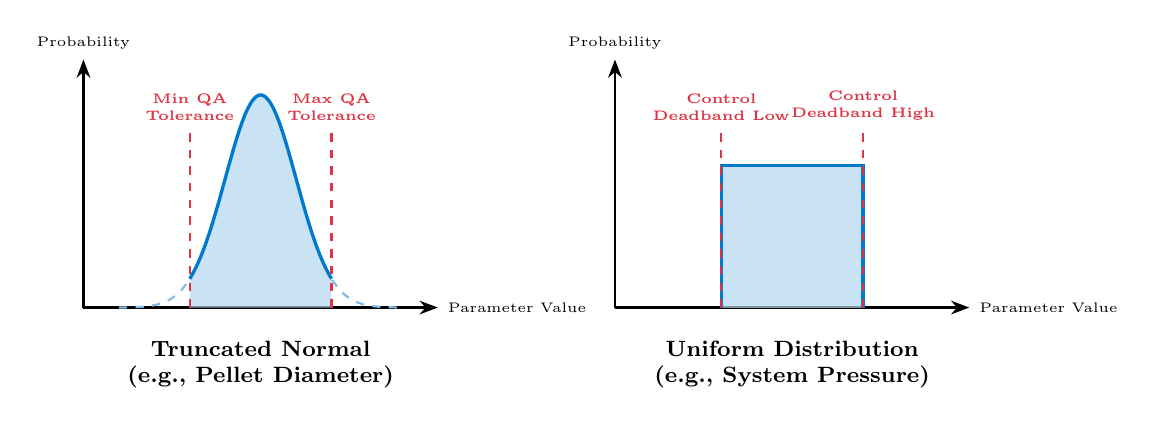
\begin{tikzpicture}[scale=0.9, every node/.style={font=\small}]
        
        % --- LEFT PLOT: Truncated Normal (Manufacturing) ---
        \begin{scope}[xshift=0cm]
            \draw[-Stealth, thick] (0,0) -- (5,0) node[right, font=\tiny] {Parameter Value};
            \draw[-Stealth, thick] (0,0) -- (0,3.5) node[above, font=\tiny] {Probability};
            
            % Full Normal Curve (light/dashed)
            \draw[dashed, HadronBlue!50, thick] plot[domain=0.5:4.5, samples=50] (\x, {3*exp(-2*(\x-2.5)^2)});
            
            % Truncated Filled Area
            \fill[HadronBlue!30, opacity=0.7] plot[domain=1.5:3.5, samples=50] (\x, {3*exp(-2*(\x-2.5)^2)}) -- (3.5,0) -- (1.5,0) -- cycle;
            
            % Solid Curve for Truncated part
            \draw[very thick, HadronBlue] plot[domain=1.5:3.5, samples=50] (\x, {3*exp(-2*(\x-2.5)^2)});
            
            % Cutoff lines
            \draw[dashed, StatusRed, thick] (1.5,0) -- (1.5,2.5) node[above, font=\tiny\bfseries, align=center] {Min QA\\Tolerance};
            \draw[dashed, StatusRed, thick] (3.5,0) -- (3.5,2.5) node[above, font=\tiny\bfseries, align=center] {Max QA\\Tolerance};
            
            \node[font=\footnotesize\bfseries, align=center] at (2.5, -0.8) {Truncated Normal\\(e.g., Pellet Diameter)};
        \end{scope}

        % --- RIGHT PLOT: Uniform (Operating Conditions) ---
        \begin{scope}[xshift=7.5cm]
            \draw[-Stealth, thick] (0,0) -- (5,0) node[right, font=\tiny] {Parameter Value};
            \draw[-Stealth, thick] (0,0) -- (0,3.5) node[above, font=\tiny] {Probability};
            
            % Uniform Box
            \fill[HadronBlue!30, opacity=0.7] (1.5,0) rectangle (3.5, 2.0);
            \draw[very thick, HadronBlue] (1.5,0) -- (1.5,2.0) -- (3.5,2.0) -- (3.5,0);
            
            % Cutoff lines
            \draw[dashed, StatusRed, thick] (1.5,0) -- (1.5,2.5) node[above, font=\tiny\bfseries, align=center] {Control\\Deadband Low};
            \draw[dashed, StatusRed, thick] (3.5,0) -- (3.5,2.5) node[above, font=\tiny\bfseries, align=center] {Control\\Deadband High};
            
            \node[font=\footnotesize\bfseries, align=center] at (2.5, -0.8) {Uniform Distribution\\(e.g., System Pressure)};
        \end{scope}
        
    \end{tikzpicture}
    \end{center}
    
    \vspace{0.5em}
    \statusbadge{HadronDark}{Rule: Never sample physically impossible states. Tail truncation is required.}
\end{frame}

% ==========================================
% SLIDE 11: CATEGORY 1: MANUFACTURING
% ==========================================
\begin{frame}[t]{Category 1: Manufacturing Tolerances}
    \begin{columns}[T,onlytextwidth]
        \column{0.55\textwidth}
        \textbf{Fuel and Core Geometry}
        The Approach: Do not guess these; rely on the actual Quality Assurance/Quality Control (QA/QC) data from the fuel fabrication facility.
        \begin{itemize}
            \item \textit{Examples:} Pellet enrichment, theoretical density, clad outer diameter, fuel rod pitch.
        \end{itemize}

        \column{0.40\textwidth}
        \begin{block}{PDF Selection Rules}
            \begin{itemize} \small
                \item \textbf{Truncated Normal:} QA data forms a Gaussian curve, but QA rejects items outside tolerance bands. Truncate the PDF to avoid impossible configurations.
                \item \textbf{Uniform:} If historical QA data is lacking (e.g., novel LEU+ fuel), the NRC expects a Uniform distribution between min/max limits.
            \end{itemize}
        \end{block}
    \end{columns}
\end{frame}

% ==========================================
% SLIDE 12: CATEGORY 2: OPERATING CONDITIONS
% ==========================================
\begin{frame}[t]{Category 2: Operating Conditions}
    \begin{columns}[T,onlytextwidth]
        \column{0.55\textwidth}
        \textbf{Plant State and Boundary Conditions}
        The Approach: Base these strictly on the reactor's Technical Specifications, instrument uncertainties, and control system deadbands.
        \begin{itemize}
            \item \textit{Examples:} Core thermal power, primary pump mass flow rate, core inlet temperature, system pressure.
        \end{itemize}

        \column{0.40\textwidth}
        \begin{block}{PDF Selection Rules}
            \begin{itemize} \small
                \item \textbf{Normal:} Used for instrument errors. If a thermocouple is accurate to $\pm 2^\circ$F (95\% confidence), map to a Normal distribution where $2\sigma = 2^\circ$F.
                \item \textbf{Uniform:} Used for control bands. If automated systems allow pressure to float between 1490 and 1510 psia before actuating, use Uniform across that 20 psi band.
            \end{itemize}
        \end{block}
    \end{columns}
\end{frame}

% ==========================================
% SLIDE 13: CATEGORY 3: MODELING UNCERTAINTIES
% ==========================================
\begin{frame}[t]{Category 3: Modeling Uncertainties}
    \begin{columns}[T,onlytextwidth]
        \column{0.55\textwidth}
        \textbf{Code and Correlation Flaws}
        The most difficult category. No computer code is perfect. You must quantify how wrong your Evaluation Models are when compared to actual physical experiments.
        \begin{itemize}
            \item \textit{Examples:} Heat transfer coefficients, two-phase friction multipliers, gap conductance models.
        \end{itemize}
        
        \vspace{1em}
        \textbf{The Approach:}
        Simulate historical validation tests and plot \textbf{Predicted vs. Measured} results.

        \column{0.40\textwidth}
        \begin{block}{PDF Selection Rules}
            \begin{itemize} \small
                \item \textbf{Bias \& Variance:} Data scatter provides the standard deviation; consistent over/under-prediction provides the "bias".
                \item \textbf{Lognormal:} Often required if a parameter strictly cannot be less than zero (e.g., friction multipliers).
            \end{itemize}
        \end{block}
    \end{columns}
\end{frame}

% ==========================================
% SLIDE 14: STEP 3: CORRELATIONS
% ==========================================
\begin{frame}[t]{Step 3: Checking for Parameter Correlations}
    \textbf{The Trap of Independence:}
    A common trap in BEPU analysis is treating all variables as completely independent. If your statistical sampler randomly picks values without knowing they are related, it will simulate physically impossible reactors.

    \vspace{1em}
    \begin{columns}[T,onlytextwidth]
        \column{0.48\textwidth}
        \begin{block}{The Problem}
            \textbf{Example:} Fuel pellet density and fuel pellet diameter are often inversely correlated in manufacturing. Sampling a maximum diameter and a maximum density simultaneously could exceed the total allowed uranium mass per rod.
        \end{block}

        \column{0.48\textwidth}
        \begin{block}{The Fix}
            Construct a \textbf{covariance matrix}. When programming the sampling engine (like DAKOTA or RAVEN), input the covariance matrix so that if it samples a high diameter, it restricts the available sample space for density.
        \end{block}
    \end{columns}
\end{frame}

% ==========================================
% SLIDE 15: STEP 4: JUSTIFICATION
% ==========================================
\begin{frame}[t]{Step 4: The PDF Justification Document}
    For NRC licensing under RG 1.203, every single PDF must have a heavily documented "pedigree." 

    \vspace{1em}
    \textbf{The Uncertainty Quantification Report:}
    This document must detail the following for every parameter fed into the engine:
    \begin{enumerate}
        \item \textbf{Definition:} What the parameter is.
        \item \textbf{PIRT Rank:} Why it was ranked High importance.
        \item \textbf{Raw Data Source:} E.g., "Vendor QA report 2024," "Instrument Cal-Spec," or "Validation Test Suite B".
        \item \textbf{Mathematical Fit:} E.g., Normal, $\mu=1500$, $\sigma=4.5$.
        \item \textbf{Goodness-of-Fit Test:} E.g., Passing a Shapiro-Wilk test to mathematically prove the data actually fits the chosen PDF.
    \end{enumerate}
\end{frame}

% ==========================================
% SLIDE 16: INTRO TO COMBINATION
% ==========================================
\begin{frame}[t]{The Challenge of Combining Uncertainties}
    \textbf{The Objective:}
    Once individual PDFs for all High-Ranked PIRT parameters are justified, they must be mathematically combined to yield a single total uncertainty statement for the Figure of Merit (FOM).

    \vspace{1em}
    \begin{columns}[T,onlytextwidth]
        \column{0.50\textwidth}
        \textbf{Why is this difficult?}
        \begin{itemize}
            \item \textbf{Non-linearity:} Reactor transients are highly non-linear. Doubling an input error does not simply double the output error.
            \item \textbf{Synergistic Effects:} Parameters interact during an accident (e.g., pump flow and decay heat interacting with system pressure).
        \end{itemize}

        \column{0.45\textwidth}
        \begin{block}{Methods of Combination}
            \begin{enumerate}
                \item Square Root of Sum of Squares (SRSS)
                \item Response Surface Methodology (RSM)
                \item Direct Monte Carlo Sampling
            \end{enumerate}
        \end{block}
    \end{columns}
\end{frame}

% ==========================================
% SLIDE 17: METHOD 1: SRSS
% ==========================================
\begin{frame}[t]{Combination Method 1: SRSS}
    \begin{columns}[T,onlytextwidth]
        \column{0.55\textwidth}
        \textbf{Square Root of the Sum of the Squares (SRSS)}
        The traditional, simplistic method for combining statistical variations.
        
        \[ U_{total} = \sqrt{ U_1^2 + U_2^2 + U_3^2 + \dots + U_n^2 } \]

        \vspace{1em}
        \textbf{Limitations for BEPU:}
        \begin{itemize}
            \item \textbf{Strict Independence:} It assumes parameters do not influence each other. 
            \item \textbf{Linearity Assumption:} It assumes the output responds linearly to inputs, which is rarely true in complex nuclear safety transients (e.g., LOCA).
        \end{itemize}

        \column{0.40\textwidth}
        \vspace{1em}
        \statusbadge{StatusRed}{Rarely accepted for complex EMs}
        \vspace{1em}
        \small \textit{NRC Note:} RG 1.203 requires extensive justification if linear SRSS is used to combine phenomenological uncertainties.
    \end{columns}
\end{frame}

% ==========================================
% SLIDE 18: METHOD 2: RESPONSE SURFACES
% ==========================================
\begin{frame}[t]{Combination Method 2: Response Surface Methodology}
    \textbf{Response Surface Methodology (RSM)}
    Used historically when running a full-scale Evaluation Model 10,000 times was too computationally expensive.

    \vspace{1em}
    \begin{columns}[T,onlytextwidth]
        \column{0.48\textwidth}
        \begin{block}{The Process}
            \begin{enumerate} \small
                \item Run the EM a limited number of times using an experimental design (e.g., Latin Hypercube).
                \item Fit a mathematical surrogate model (polynomial) to the outputs.
                \item Perform Monte Carlo sampling on the \emph{fast surrogate}, not the slow EM.
            \end{enumerate}
        \end{block}

        \column{0.48\textwidth}
        \textbf{Drawbacks:}
        \begin{itemize} \small
            \item The surrogate polynomial may fail to capture sudden cliff-edge effects (which are common in multi-phase flow).
            \item Introduces an extra layer of "fitting uncertainty" that must be quantified.
        \end{itemize}
    \end{columns}
\end{frame}

% ==========================================
% SLIDE 19: METHOD 3: MONTE CARLO
% ==========================================
\begin{frame}[t]{Combination Method 3: Direct Monte Carlo Sampling}
    \begin{columns}[T,onlytextwidth]
        \column{0.65\textwidth}
        \textbf{The Modern Standard:}
        With modern computing clusters, we bypass surrogates and directly sample the physics code. 
        
        \vspace{1em}
        \textbf{How it works:}
        A sampling engine (like DAKOTA or RAVEN) randomly pulls values from all defined input PDFs simultaneously, passes them to the Evaluation Model, runs the transient, and records the Figure of Merit.

        \vspace{1em}
        \statusbadge{StatusGreen}{Advantage: Naturally captures all non-linear physics and correlations.}

        \column{0.30\textwidth}
        \begin{block}{Requirements}
            Requires vast computational resources, but eliminates surrogate fitting errors.
        \end{block}
    \end{columns}
\end{frame}

% ==========================================
% SLIDE 20: WILKS FORMULA
% ==========================================
\begin{frame}[t]{Non-Parametric Order Statistics (Wilks' Formula)}
    \textbf{The Question:} How many times ($N$) must we run the Monte Carlo simulation to prove safety?

    \vspace{1em}
    \begin{columns}[T,onlytextwidth]
        \column{0.50\textwidth}
        \textbf{Wilks' Theorem:}
        Allows us to determine the tolerance limit of a distribution without knowing the shape of that distribution (non-parametric). 
        
        \vspace{0.5em}
        Crucially, the required number of runs ($N$) is \textbf{independent of the number of input parameters}.

        \column{0.45\textwidth}
        \begin{block}{Common $N$ Values (95/95 Limit)}
            \begin{itemize} \small
                \item \textbf{1st Order ($N=59$):} The worst-case result out of 59 runs bounds 95\% of the population with 95\% confidence.
                \item \textbf{2nd Order ($N=93$):} The second-worst result out of 93 runs bounds the 95/95 limit.
                \item \textbf{3rd Order ($N=124$).}
            \end{itemize}
        \end{block}
    \end{columns}
\end{frame}

% ==========================================
% SLIDE 21: THE 95/95 LIMIT (TIKZ)
% ==========================================
\begin{frame}[t]{Establishing the 95/95 Safety Limit (Monte Carlo)}
    \vspace{1em}
    \begin{center}
    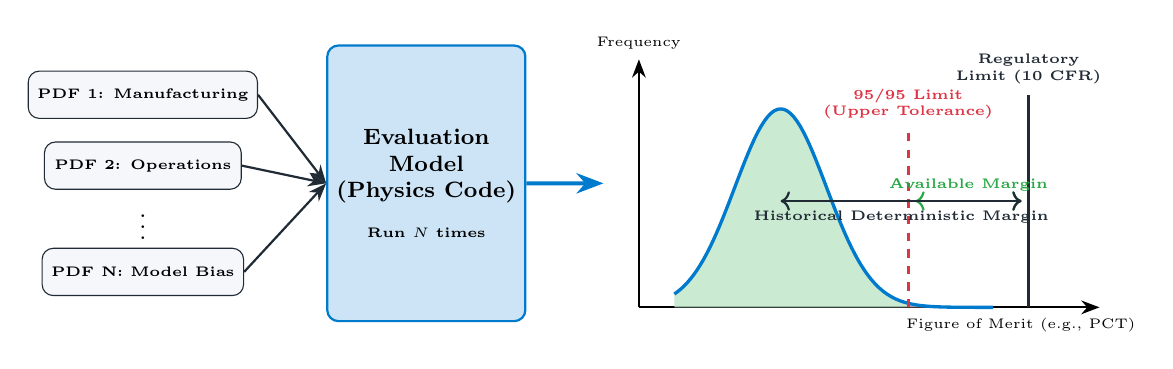
\begin{tikzpicture}[scale=0.9, every node/.style={font=\small}]
        
        % --- INPUT PDFs ---
        \node[draw=HadronDark, fill=HadronLight, rounded corners, minimum height=0.6cm, minimum width=2.5cm, font=\tiny\bfseries] (in1) at (0, 2.5) {PDF 1: Manufacturing};
        \node[draw=HadronDark, fill=HadronLight, rounded corners, minimum height=0.6cm, minimum width=2.5cm, font=\tiny\bfseries] (in2) at (0, 1.5) {PDF 2: Operations};
        \node at (0, 0.75) {$\vdots$};
        \node[draw=HadronDark, fill=HadronLight, rounded corners, minimum height=0.6cm, minimum width=2.5cm, font=\tiny\bfseries] (inN) at (0, 0) {PDF N: Model Bias};

        % --- EVALUATION MODEL ---
        \node[draw=HadronBlue, fill=HadronBlue!20, thick, rounded corners, minimum height=3.5cm, minimum width=2.5cm, align=center, font=\footnotesize\bfseries] (code) at (4, 1.25) {Evaluation\\Model\\(Physics Code)\\[0.5em] \tiny Run $N$ times};

        % Arrows In
        \draw[-Stealth, thick, HadronDark] (in1.east) -- (code.west);
        \draw[-Stealth, thick, HadronDark] (in2.east) -- (code.west);
        \draw[-Stealth, thick, HadronDark] (inN.east) -- (code.west);

        % Arrow Out
        \draw[-Stealth, thick, HadronBlue, line width=1.5pt] (code.east) -- (6.5, 1.25);

        % --- OUTPUT DISTRIBUTION ---
        \begin{scope}[xshift=7cm, yshift=-0.5cm]
            \draw[-Stealth, thick] (0,0) -- (6.5,0) node[below, xshift=-1cm, font=\tiny] {Figure of Merit (e.g., PCT)};
            \draw[-Stealth, thick] (0,0) -- (0,3.5) node[above, font=\tiny] {Frequency};
            
            % Curve & Shading (Left 95%)
            \fill[StatusGreen!30, opacity=0.8] plot[domain=0.5:3.8, samples=100] (\x, {2.8*exp(-1.2*(\x-2)^2)}) -- (3.8,0) -- (0.5,0) -- cycle;
            % Curve & Shading (Right 5% - Tail)
            \fill[StatusRed!30, opacity=0.8] plot[domain=3.8:5.0, samples=100] (\x, {2.8*exp(-1.2*(\x-2)^2)}) -- (5.0,0) -- (3.8,0) -- cycle;
            
            \draw[very thick, HadronBlue] plot[domain=0.5:5.0, samples=100] (\x, {2.8*exp(-1.2*(\x-2)^2)});
            
            % Lines
            \draw[dashed, very thick, StatusRed] (3.8, 0) -- (3.8, 2.5) node[above, font=\tiny\bfseries, align=center] {95/95 Limit\\(Upper Tolerance)};
            \draw[very thick, HadronDark] (5.5, 0) -- (5.5, 3.0) node[above, font=\tiny\bfseries, align=center] {Regulatory\\Limit (10 CFR)};
            
            % Margin Arrow
            \draw[<->, thick, StatusGreen] (3.9, 1.5) -- (5.4, 1.5) node[midway, above, font=\tiny\bfseries] {Available Margin};
            \draw[<->, thick, HadronDark] (2.0, 1.5) -- (5.4, 1.5) node[midway, below, font=\tiny\bfseries] {Historical Deterministic Margin};
            
        \end{scope}
    \end{tikzpicture}
    \end{center}
    
    \vspace{0.5em}
    \statusbadge{HadronBlue}{BEPU Benefit: Safely recovering margin previously lost to deterministic assumptions.}
\end{frame}

% ==========================================
% SLIDE 22: SUMMARY & REFERENCES
% ==========================================
\begin{frame}[t]{Summary \& References}
    \begin{columns}[T,onlytextwidth]
        \column{0.55\textwidth}
        \textbf{The BEPU Philosophy:}
        RG 1.203 shifts safety analysis away from unphysical assumptions toward realistic physics, bounded strictly by mathematically combined uncertainty matrices.

        \vspace{1em}
        \begin{block}{NRC Submittal Checklist}
            \begin{enumerate} \small
                \item Is the PIRT complete?
                \item Are scaling distortions quantified?
                \item Are PDFs sourced from QA or Test data?
                \item Are correlations defined via covariance?
                \item Is uncertainty quantified and combined to the 95/95 limit?
            \end{enumerate}
        \end{block}

        \column{0.40\textwidth}
        \textbf{Key Regulatory Resources}
        \begin{itemize} \small
            \item Regulatory Guide 1.203, \emph{Transient and Accident Analysis Methods}.
            \item NUREG/CR-5249, \emph{Quantifying Reactor Safety Margins} (CSAU).
        \end{itemize}
        
        \vspace{1em}
        \textbf{Industry Tools}
        \vspace{0.5em} \\
        \statusbadge{HadronBlue}{RELAP5-3D} \vspace{0.3em} \\
        \statusbadge{HadronBlue}{TRACE} \vspace{0.3em} \\
        \statusbadge{HadronBlue}{RAVEN / DAKOTA}
    \end{columns}
\end{frame}

\end{document}
